\chapter{Reconstruction}
\label{ch:reconstruction}

Each event within an AD is assigned a reconstructed position and energy
that take into account the pattern of PMT hits, the total light emitted,
scintillator and mineral oil optical characteristics,
spatial nonuniformity, and scintillator and electronics nonlinearity.
The reconstructed positions are used to compute the distance-time cut
to select IBD events as described in \cref{sec:DT_cut},
and are also used as inputs to the energy reconstruction
to help correct for nonuniformities in the ADs' light collection
as a function of position.
The reconstructed energy is a critical input to the \thetaot{} analysis
due to the heavy reliance on energy cuts to select IBDs and reject background.
The relative performance of ADs in reconstructing energy
is particularly important, since inconsistencies in energy reconstruction
could lead to unaccounted-for differences in efficiency,
which would bias the measurement of \thetaot.
The position reconstruction procedure will be detailed in \cref{sec:reco_position}.
Energy reconstruction, including the energy scale, determination of event energy,
and the nonuniformity and nonlinearity corrections,
will be described in \cref{sec:reco_energy}.

\section{Position}
\label{sec:reco_position}

Daya Bay uses two independent position reconstruction algorithms,
both of which rely on the pattern of charge measurements across all PMTs in an AD.
The reconstruction used in this \thetaot{} analysis is known as ``AdSimple;''
the name was inherited from a predecessor algorithm \cite{adsimple1}.
The other reconstruction is called ``AdScaled.''

In AdScaled, a center-of-charge position is computed,
averaging over each PMT position weighted by the charge on the PMT,
and a parametrized correction derived from simulation
is applied to determine the reconstructed position \cite{ngd2016}.
However, AdSimple was determined to be the best for use in the nH analysis.

In AdSimple,
each event's PMT charge pattern is compared to a library of \num{9600} templates
generated using a Monte Carlo simulation.
Each template represents one position on an $(r, \phi, z)$ grid
with \num{20} $r$ positions, \num{24} $\phi$ positions,
and \num{20} $z$ positions.
A $\chi^2$ is constructed to quantify the agreement between the measured charge pattern
and each of the templates:

\begin{equation}
    \chi^2(\textbf{r}_{\text{rec}}) = \sum_{i=1}^{192} -2\ln\frac{
        \text{Poisson}(N_i^{\text{obs}} \vert N_i^{\text{template}}(\textbf{r}_{\text{rec}}))
    }
    {
        \text{Poisson}(N_i^{\text{obs}} \vert N_i^{\text{obs}})
    },
\end{equation}
where $i$ indexes over PMTs,
$N_i^{\text{obs}}$ is the number of photoelectrons observed in PMT $i$,
$N_{i}^{\text{template}}(\textbf{r}_{\text{rec}})$ is the prediction
for PMT $i$ of the template for reconstructed position $\textbf{r}_{\text{rec}}$,
and $\text{Poisson}(n\vert\mu)$ is the Poisson probability
to observe $n$ counts given an expected value of $\mu$.
Once the lattice point with the least $\chi^2$ is found,
an interpolation is performed along each coordinate dimension $(r, \phi, z)$
as depicted in \cref{fig:interpolation}
to extend the domain of the $\chi^2$ function to all positions within the AD,
not just the lattice points.
The value of $\textbf{r}_{\text{rec}}$ which minimizes $\chi^2$
is used as the reconstructed position.
The distribution of reconstructed positions is shown in \cref{fig:position_map},
with artifacts of the interpolation process clearly visible.

\todo[inline]{Diagram here or in Detector chapter showing coordinate system}

\begin{figure}
    \centering
    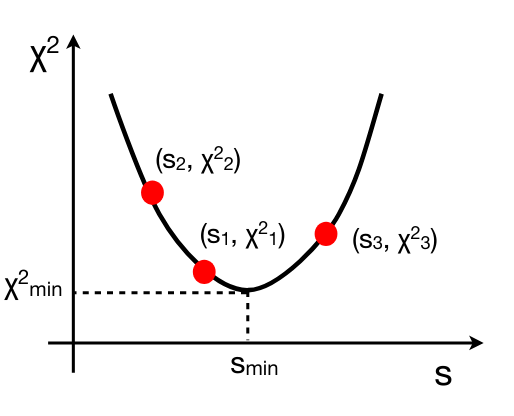
\includegraphics[width=0.4\textwidth]{ch_reconstruction/interpolation}
    \caption{
        Interpolation between grid points to obtain a more-precise position
        that minimizes the $\chi^2$ function.
        The process is repeated with $s$ representing each of the coordinates
        $r, \phi, z$.
        Figure taken from \cite{adsimple1}.
    }
    \label{fig:interpolation}
\end{figure}

\begin{figure}
    \missingfigure{Reconstructed position distribution for events in EH1-AD1}
    \caption{
        Reconstructed positions of events with energy within \SIrange{1.5}{12}{\MeV}
        in EH1-AD1.
    }
    \label{fig:position_map}
\end{figure}

\section{Energy}
\label{sec:reco_energy}

The reconstructed energy for an event is built up from the previously-described
calibration values and the observed signals in each PMT.
PMT observed ADC values are converted into charges using the gain
and corrected for the single-channel nonlinearity.
The total charge on all PMTs is converted into an energy value
using the light yield measured during calibration,
and then corrected to account for any disabled PMTs
and for variations in the detector response as a function of position and time.
This process can be represented by the following formula:

\begin{equation}
    E_{\text{rec}} = \left(
        \sum_i f_{\text{SCNL}}\left(\frac{Q_i}{\overline{Q}_i^{\text{SPE}}(t)}\right)
    \right)
    \frac{f_{\text{act}}(t)}{N^{\text{PE}}(t)}
    f_{\text{pos}}(\textbf{r}_{\text{rec}},t),
\end{equation}
where $Q_i$ is the ADC value for PMT $i$,
$\overline{Q}_i^{\text{SPE}}(t)$ and $N^{\text{PE}}(t)$
are the gain for PMT $i$ and the light yield, respectively
(\cref{sec:gain,sec:light_yield_calib}),
$f_{\text{SCNL}}$ is the single-channel nonlinearity correction
(\cref{subsec:scnl}),
and $f_{\text{act}}(t)$ and $f_{\text{pos}}(\textbf{r}_{\text{rec}},t)$
are the active PMT correction and nonuniformity correction,
described below.

The active PMT correction compensates for the loss in collected light
when a PMT must be disabled during operation \cite{ngd2016}.
On average, each PMT contributes $\nicefrac{1}{192}$ of the charge to each event.
Thus if $n$ PMTs are disabled, the measured total charge must be increased by a factor

\begin{equation}
    f_{\text{act}}(n) = \frac{192}{n}.
\end{equation}
The correction is time-dependent since the number of disabled PMTs changes with time.
\todo{Decide whether to study improved active PMT correction}

The rest of this chapter will describe the
nonuniformity correction $f_{\text{pos}}(\textbf{r}_{\text{rec}},t)$
(\cref{subsec:nonuniformity})
as well as characterizations of the detector energy response:
the energy resolution (\cref{subsec:resolution}),
relative energy scale (\cref{subsec:rel_energyscale}),
and absolute energy scale (\cref{subsec:abs_energyscale}).

\subsection{Nonuniformity correction}
\label{subsec:nonuniformity}

The nonuniformity correction ensures that events of a given physical energy
occurring in different regions of the AD
are assigned the same reconstructed energy.
Nonuniformities in reconstructed energy arise due to a variety of factors
including PMT light acceptance as a function of incident angle;
optical properties of the scintillator, mineral oil, and acrylic vessels;
and the orientation of PMTs with respect to the Earth's magnetic field.
The nonuniformity correction is factored into corrections based on
$r$ and $z$ position, azimuthal angle $\phi$, and time
(which also has a radial dependence):
\begin{equation}
    f_{\text{pos}}(\textbf{r}_{\text{rec}},t) =
    f_{\text{pos}}(r, z)f_{\text{pos}}(\phi)f_{\text{pos}}(r, t).
\end{equation}

Maps for the $r$--$z$ nonuniformity were constructed for each AD
by identifying neutron captures on both Gd and H,
and comparing the energy of events in a given region of the AD
to the average of the entire AD.
The AD was divided into equal-volume concentric rings
represented as squares on a plot of $z$ vs. $r^2$.
Neutron captures of spallation neutrons were selected
based on a time coincidence with a previous muon signal in the AD.
Neutron captures with energy near \SI{8}{\MeV} were assumed to be nGd captures,
and those with energy near \SI{2.2}{\MeV} were assumed to be nH.
The peak value was extracted from a fit of the respective distributions
for each pixel and for the entire sample.
\todo{What is the ``average'' value for LS pixels?}
The nGd peak was fit with a double-Crystal Ball function \cite{cbfunction},
\todo[inline]{Describe CB function here or in Calibration chapter}
and the nH peak was fit with a calorimeter function \cite{calorimeter2016}
(described in \cref{subsec:delayed}).
A correction was then applied to each event's energy based on its position:
\begin{equation}
    f_{\text{pos}}(r, z) = \frac{E_{\text{avg}}}{E_{\text{pixel}}(r,z)}.
\end{equation}
\Cref{fig:nonuniformity_map} shows the corrections $f_{\text{pos}}$ for EH1-AD1.
All ADs had similar nonuniformities, but separate corrections were still computed
for each AD.
Within an AD, the nonuniformity correction was as large as \SI{20}{\percent}
at the outer edge of the OAV (LS region).

\begin{figure}
    \centering
    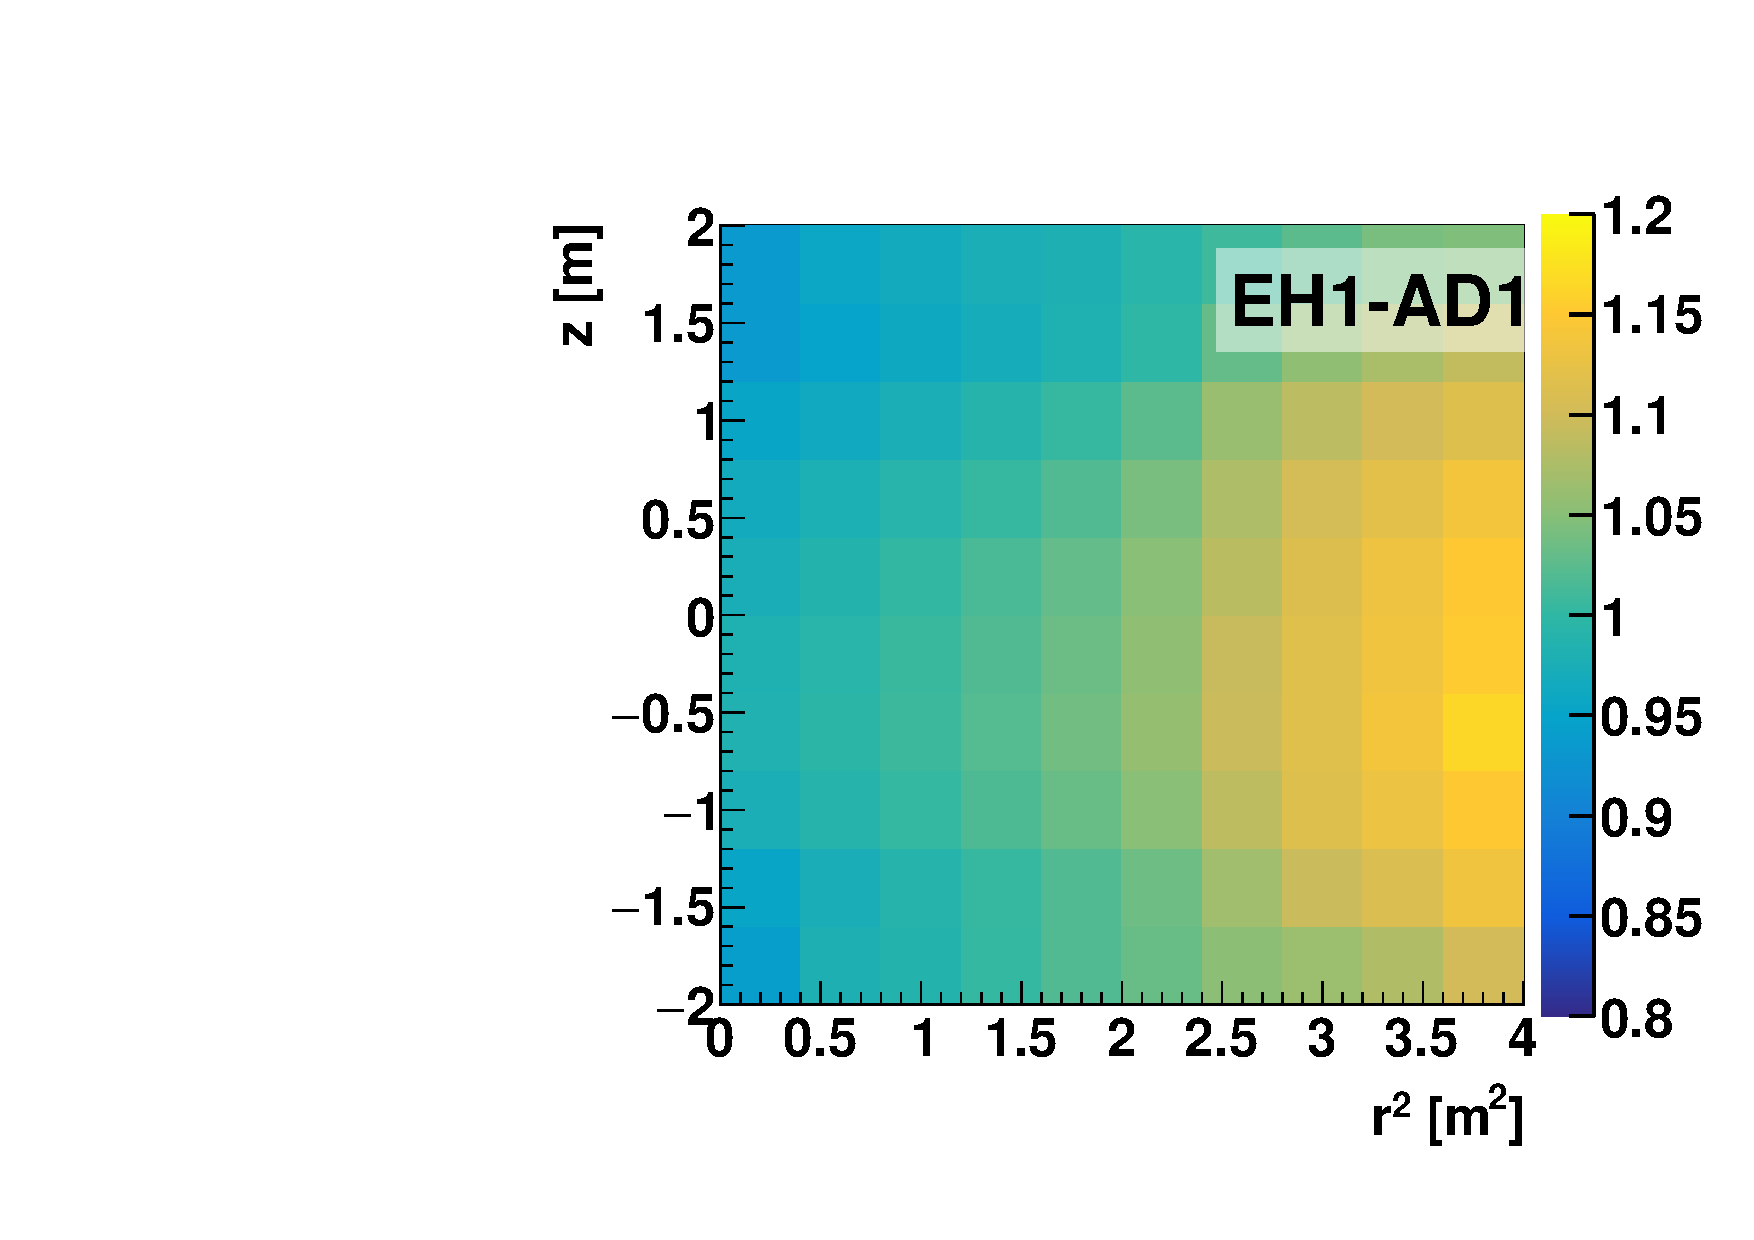
\includegraphics[width=0.4\textwidth]{ch_reconstruction/nonuniformity_map}
    \caption{
        Nonuniformity corrections based on the energy of spallation neutrons
        capturing on Gd and H.
        Plot based on data from \cite{nonuniformity2}.
        \todo[inline]{Try to find 3D contour map of nonuniformity}
    }
    \label{fig:nonuniformity_map}
\end{figure}

The Earth's magnetic field caused a nonuniformity
as a function of azimuthal angle $\phi$ of approximately \SI{1}{\percent}.
This effect was correlated with the orientation of the PMTs with respect
to the geomagnetic field.
A model was constructed to account for this effect:
\begin{equation}
    f_{\text{pos}}(\phi) = 1 + \alpha\sin(\phi-\phi_0),
\end{equation}
where $\alpha$ and $\phi_0$ were determined from fitting to spallation neutron captures
in a similar fashion as with the $r$--$z$ nonuniformity.

Over time, the nonuniformity evolved in different regions of the ADs,
attributable mostly to a slight degradation in the attenuation length of the LS
and GdLS \cite{nonuniformity3}.
The evolution was quantified by examining the spallation neutron capture energy
as a function of radial position and time.
As shown in \cref{fig:time_dep_nonunif}, a clear linear change is visible
for each bin of radial position \cite{nonuniformity1}, which was parametrized as
\begin{equation}
    f_{\text{pos}}(t, r) = (\beta_0 + \beta_1r^2)t.
\end{equation}
All ADs showed a similar trend, so a combined fit was performed,
yielding values of $\beta_0 + \beta_1r^2$ between
\SIlist[retain-explicit-plus]{-0.12;+0.4}{\percent} per year.

\begin{figure}
    \centering
    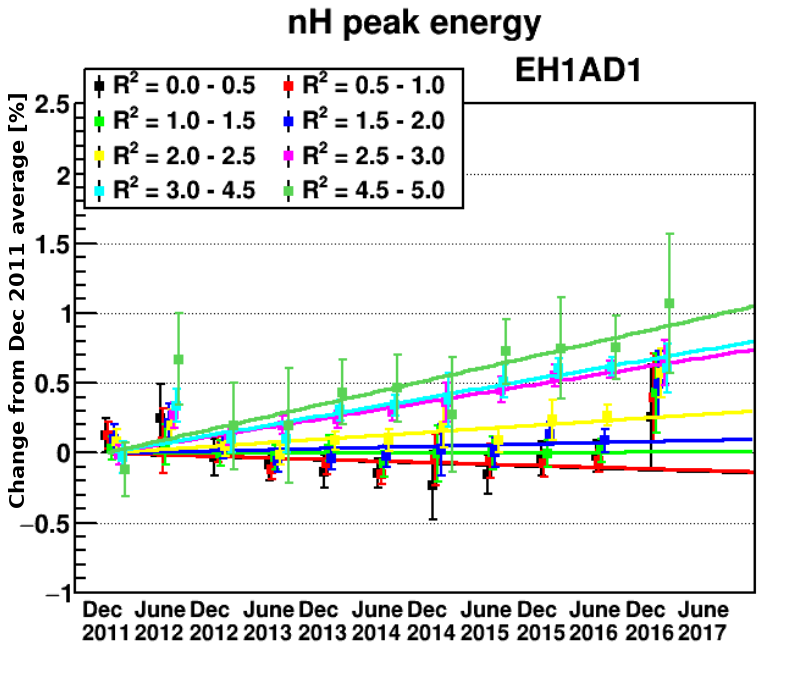
\includegraphics[width=0.8\textwidth]{ch_reconstruction/time_dep_nonunif}
    \caption{
        Relative change over time in energy for spallation neutrons capturing on H.
        Each color is a different range of event radius.
        The correction coefficients $\beta_0$ and $\beta_1$ are determined
        from a fit of the slope as a function of radius.
        Figure taken from \cite{nonuniformity4}.
        \todo[inline]{Photoshop yellow line to a different color}
        \todo[inline]{Add table showing $\beta_{0,1}$ for each AD, if available}
    }
    \label{fig:time_dep_nonunif}
\end{figure}

\subsection{Energy resolution}
\label{subsec:resolution}

The detector energy resolution for a scintillating detector can be modeled as
\cite{energy_resolution}

\begin{equation}
    \frac{\sigma_E}{E} = \sqrt{a^2 + \frac{b^2}{E} + \frac{c^2}{E^2}},
\end{equation}
where $E$ is the reconstructed energy.
The parameters $a,b,$ and $c$ represent contributions to the resolution
from different sources.
Parameter $a$ quantifies the impact due to the non-pointlike nature
of the energy depositions in the scintillator,
since events with larger energy deposit their energy over a larger spatial extent
in the AD.
This could also be understood as a consequence of residual nonuniformity.
Parameter $b$ describes the size of the $\nicefrac{1}{\sqrt{E}}$ contribution,
which corresponds to the combined counting statistics of
the production, detection and digitization of photons.
Lastly, $c$ is a constant contribution to $\sigma_E$
representing the dark noise intrinsic to the PMTs.
The resolution parameters can be extracted from a fit
to the energy resolutions of a wide variety of calibration and intrinsic sources,
as shown in \cref{fig:resolution}.
The values for the resolution parameters are \todo[inline]{Resolution parameter values}.

\begin{figure}
    \missingfigure{Resolution fit plot}
    \caption{Energy resolutions for calibration sources, neutron captures,
        and natural $\alpha$'s present in the ADs.%
    }
    \label{fig:resolution}
\end{figure}


\subsection{Relative energy scale}
\label{subsec:rel_energyscale}

It is critical that all ADs measure the same energy when observing the same process.
If an AD is biased and returns a higher or lower energy than the others,
then the IBD selection efficiency and spectral shape for that AD
may be different than at the other ADs,
which would bias the measurement of \thetaot{} and \dmee{}.
The identicalness of the energy measurements is known as the relative energy scale,
and it is determined by measuring the same process in all ADs and comparing
the reconstructed energy.
The energy scale of the GdLS region is extremely well-constrained
by a thorough review of 13 calibration and intrinsic sources:
$\gamma$-rays from \isotope[68]{Ge} and \isotope[60]{Co} calibration sources;
neutron captures on Gd and H from both IBD and muon spallation;
$\alpha$ decays of naturally-occuring \isotope[212]{Po},
\isotope[214]{Po}, \isotope[215]{Po}, and \isotope[219]{Po};
and $\gamma$-rays from \isotope[40]{K} and \isotope{208}[Tl].
\todo{Add \isotope[12]{B} characterization of $\beta$'s}
\Cref{fig:gdls_rel_energyscale} shows the relative variations
for all of these sources among the 8 ADs.
The variations are all within \SI{+-0.2}{\percent}.

\begin{figure}
    \centering
    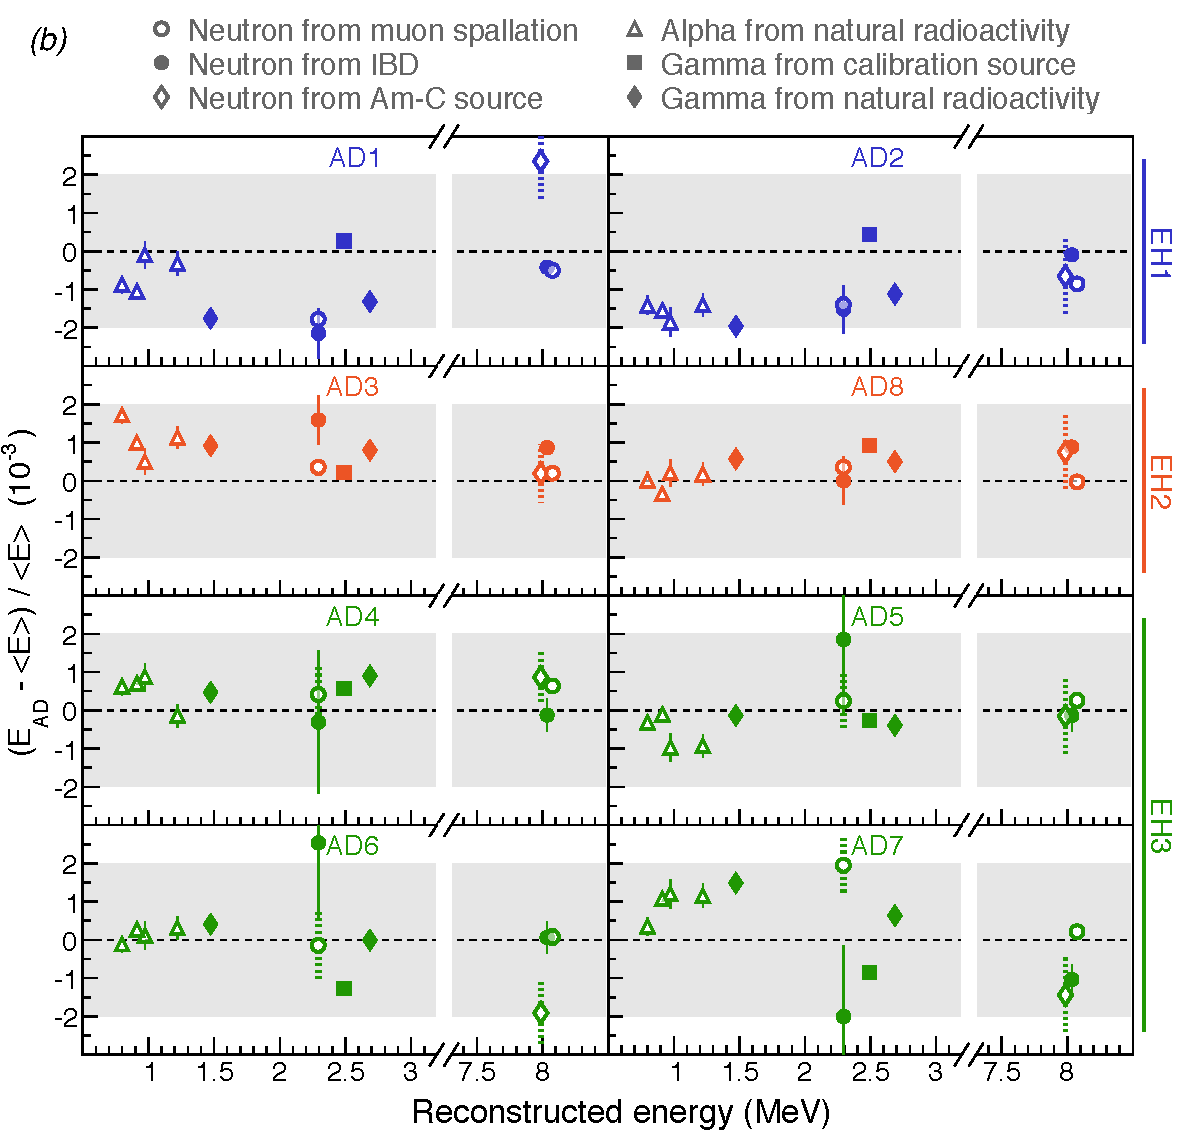
\includegraphics[width=0.9\textwidth]{ch_reconstruction/relative_energyscale}
    \caption{
        Comparison of 13 calibration and intrinsic source energies
        among the 8 ADs, showing the \SI{+-0.2}{\percent}
        relative energy scale variation in the GdLS region.
    }
    \label{fig:gdls_rel_energyscale}
\end{figure}

To include the LS region, the relative energy scale is studied
by comparing the energy of the neutron capture on H (nH)
among the ADs.
This technique is described in detail in \cref{subsec:delayed}
and results in a less-constrained relative energy scale variation
of \SI{+-0.5}{\percent}, which is conservatively adopted
as the energy scale uncertainty over the entire AD.
The impact of this variation on the prompt energy cut efficiency
and the prompt spectrum shape
is studied using simulation
as described in \cref{subsec:thu_toymc_prompt}.

\subsection{Absolute energy scale}
\label{subsec:abs_energyscale}

The calibration and reconstruction procedures discussed so far
only ensure that the ADs have nearly-identical energy responses,
and that they all assign the lower-energy $\gamma$-ray peak from nGd capture
to have energy \SI{7.95}{\MeV}.
Missing from the characterization is whether any other physical process
is assigned an accurate energy by the ADs.
That is, even if all ADs observing the same process with energy $E_{\text{true}}$
measure the same value $E_{\text{rec}}$,
how close is $E_{\text{rec}}$ to $E_{\text{true}}$?
The deviation as a function of $E_{\text{true}}$ is known as
the absolute energy scale or the absolute energy nonlinearity.

The absolute energy scale deviated from unity due to four main effects:
the IBD neutron recoil kinetic energy, scintillator quenching,
Cherenkov radiation, and electronics nonlinearity. \todo{Cite DocDBs}
The effects were factored into electronics nonlinearities
and nonlinearities in generating detectable light signals
(i.e. visible energy, $E_{\text{vis}}$):
\begin{align}
    \begin{split}
        \frac{E_{\text{rec}}}{E_{\text{true}}}
        &=
        \frac{E_{\text{rec}}}{E_{\text{vis}}}
        \frac{E_{\text{vis}}}{E_{\text{true}}} \\
        &= \beta f_{\text{electronics}}(E_{\text{vis}})
        f_{\text{scintillator}}(E_{\text{true}}),
    \end{split}
\end{align}
with neutrons, quenching, and Cherenkov radiation contributing to
$f_{\text{scintillator}}(E_{\text{true}})$,
and the arbitrary normalization $\beta$ defined so that
$E_{\text{rec}} = E_{\text{true}}$
at the nGd capture peak reference energy of \SI{7.95}{\MeV}.

The neutron recoil energy was correlated with the \nuebar{} energy,
but did not result in any scintillation or Cherenkov light.
Fortunately, the energy lost was on the order of a few \si{\keV}
so was accepted as a slight broadening of the energy resolution.

The remaining scintillator effects were modeled for electrons as
\begin{equation}
    f_{\text{scintillator}}(E_{\text{true}}) =
    f_q(E_{\text{true}};k_B) + k_Cf_C(E_{\text{true}}),
\end{equation}
where $f_q$ describes the scintillation light including the quenching effect,
$k_B$ is Birks's constant which characterizes the medium (LS)
and particle type (electron),
$k_C$ is a normalization constant,
and $f_C$ is the Cherenkov light contribution.
For an electron which deposits all of its energy into the scintillator
with energy loss per unit length $\nicefrac{dE}{dx}$,
Birks's law determines the produced scintillation light up to normalization \cite{birks}:
\begin{equation}
    f_q(E_{\text{true}});k_B) = \frac{1}{E_{\text{true}}} \int_0^{E_{\text{true}}}
    \frac{dE}{1+k_B\frac{dE}{dx}}.
\end{equation}
The Cherenkov contribution $f_C$ was determined using a Monte Carlo simulation,
and $k_C$ was chosen so that the proportion of scintillation to Cherenkov photons
was correct at $E_{\text{true}} = \SI{1}{\MeV}$.
These results were then converted for use by positrons under the assumption that
(a) electrons and positrons have identical scintillation and Cherenkov properties;
and (b) on annihilation, two additional \SI{0.511}{\MeV} $\gamma$-rays are emitted.
These $\gamma$'s as well as $\gamma$'s produced by nH, nGd and other processes
can be treated recursively
since they lose energy in the scintillator
by Compton scattering, the photoelectric effect, and pair-conversion,
and the $e^{\pm}$ generated from these processes
are described by $f_{\text{scintillator}}$.
\Cref{fig:gamma_conversion} shows the probability distributions
of the energy of $e^{\pm}$ generated by a $\gamma$-ray
and subsequent electromagnetic shower for various $\gamma$ energies,
which were used to produce effective nonlinearity models for $\gamma$-rays.

\begin{figure}
    \centering
    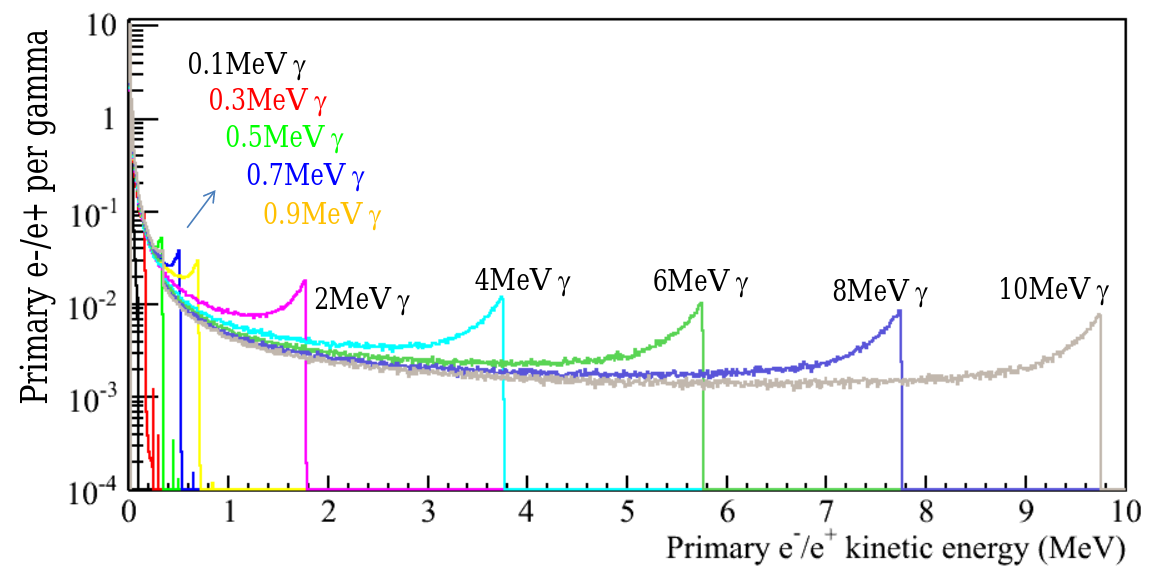
\includegraphics[width=0.9\textwidth]{ch_reconstruction/gamma_conversion_energy}
    \caption{
        Probability for a $\gamma$-ray of a given energy to produce
        an $e^{\pm}$ with a given energy in Daya Bay liquid scintillator.
        This plot was produced using Monte Carlo and is taken from \cite{nonlinearity1}.
    }
    \label{fig:gamma_conversion}
\end{figure}

The electronics nonlinearity was caused by interactions between
the timing profile of the PMT signals and the response of the readout electronics.
It was sensitive to the visible rather than true energy,
since any energy lost in the scintillator was not observed by the PMTs.
An effective model at the level of the AD rather than indivudal PMTs
was found to adequately describe the behavior:
